\subsection{Несинтаксические ограничения}
\MPS{} позволяет описывать различные несинтаксические ограничения моделей при помощи проблемно"=ориентированного языка \term{jet\-bra\-ins\-.mps\-.lang\-.const\-ra\-ints}. К таким ограничениям относятся: форматы значений свойств, функции вычисления синтетических свойств, области определения ссылок и ограничения на вложение одних узлов в другие.

Среда \MPS{} предоставляет всего три встроенных примитивных типа для свойств концептов: \term{string}, \term{boolean}, \term{integer}. Но при этом позволяет задать формат свойства и, таким образом, определить для свойства произвольный тип. Встроенный тип \term{string} разрешает использовать в качестве значения свойства любые строки. Для того, чтобы ограничить множество значений имен состояний только корректными \term{Java}-идентификаторами, концепт \term{AbstractState} реализует интерфейс"=концепт \term{IValidIdentifier}, который представляет собой раширение интерфейс"=концепта \term{INamedConcept} с соответствующим ограничением на свойство \term{name} (рис. \ref{fig:PropertyIsValid}).

\begin{figure}
 \centering
 \fbox{
  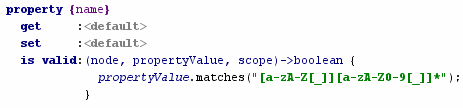
\includegraphics[width=0.8\textwidth]{PropertyIsValid.png}
 }
 \caption{Формат свойства \term{name} интерфейс"=концепта \term{IValidIdentifier}}
 \label{fig:PropertyIsValid}
\end{figure}

Любое свойство концепта может быть синтетическим, то есть вычислимым. Для этого достаточно задать функцию, вычисляющую значение этого свойства. Например, свойство \term{name} концепта \term{StateMachine} вычислимо. Его значение состоит из имени класса, автомат которого задает данный экземпляр \term{StateMachine}, и суффикса "<state machine"> (рис. \ref{fig:PropertyGet}).

\begin{figure}
 \centering
 \fbox{
  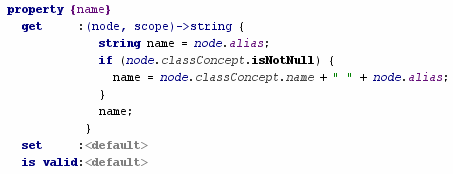
\includegraphics[width=0.8\textwidth]{PropertyGet.png}
 }
 \caption{Синтетическое свойство \term{name} концепта \term{StateMachine}}
 \label{fig:PropertyGet}
\end{figure}

При объявлении ссылки концепта кроме имени и арности указывается также целевой концепт. Этот целевой концепт определяет
множество узлов, с которыми данная ссылка может связывать узел того концепта, в котором она объявлена. По умолчанию таким
множеством будет множество всех экземпляров целевого концепта в текущей и импортированных моделях. 

Например, в концепте
\term{OutgoingTransitionAction}, соответствующем переходу из одного состояния в другое, объявлена ссылка 
\term{targetState} с целевым концептом \term{AbstractState} (рис. \ref{fig:LinkDeclaration}). Это означает, что по
умолчанию можно сделать переход из текущего состояния в любое состояние любого автомата, который найдется в данной модели
или в одной из импортированных моделей. Но это не соответствует семантике автоматного языка, потому что переходы разрешено
делать только внутри одного автомата. Для уточнения области определения ссылок в языке 
\term{jet\-bra\-ins\-.mps\-.lang\-.const\-ra\-ints} существует специальная конструкция. Эта конструкция позволяет явно задать множество узлов, с которыми может быть установлена связь. В указанном случае это все состояния, вложенные в автомат, внутри которого находится исходное состояние (рис. \ref{fig:SearchScope}).

\begin{figure}
 \centering
 \fbox{
  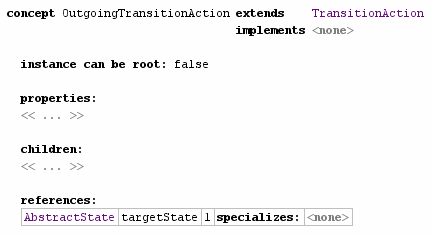
\includegraphics[width=0.9\textwidth]{LinkDeclaration.png}
 }
 \caption{Объявление ссылки \term{targetState}}
 \label{fig:LinkDeclaration}
\end{figure}

\begin{figure}
 \centering
 \fbox{
  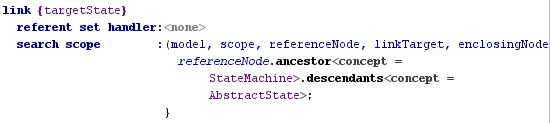
\includegraphics[width=0.9\textwidth]{SearchScope.png}
 }
 \caption{Область определения ссылки \term{targetState}}
 \label{fig:SearchScope}
\end{figure}

Также можно определить дополнительные семантические ограничения и для вложенных узлов. Концепты, указываемые при объявлении структуры вложенных узлов, синтаксически ограничивают множество концептов, экземпляры которых могут быть использованы в качестве вложенных. Конструкция \term{can be child} позволяет указать, возможно ли вложить экземпляр текущего концепта внутрь переданного в параметрах концепта. Конструкция \term{can be parent}, наоборот, позволяет указать можно ли использовать экземпляр текущего концепта в качестве родительского по отношению к концепту, переданному в параметре.